\documentclass{article}
\usepackage[utf8]{inputenc}
\usepackage{graphicx,wrapfig}
\usepackage{amsmath}
\usepackage{titling}
\usepackage{pdflscape}
\usepackage[export]{adjustbox}
\usepackage{float}
\usepackage{booktabs} % To thicken table lines
\usepackage{adjustbox}
\usepackage{caption}
\usepackage[colorlinks=false,hidelinks]{hyperref}

\setlength{\droptitle}{-4cm}
\pagestyle{empty}

\title{Lab. 5 - Clustering k-means parallelo}
\author{Ballarin Simone, Gobbo Alessio, Rossi Daniel}
\date{July 2019}

\begin{document}

\maketitle

\section*{Domanda 1}
\begin{center}
	\begin{figure}[H]
		\hspace*{1.5cm}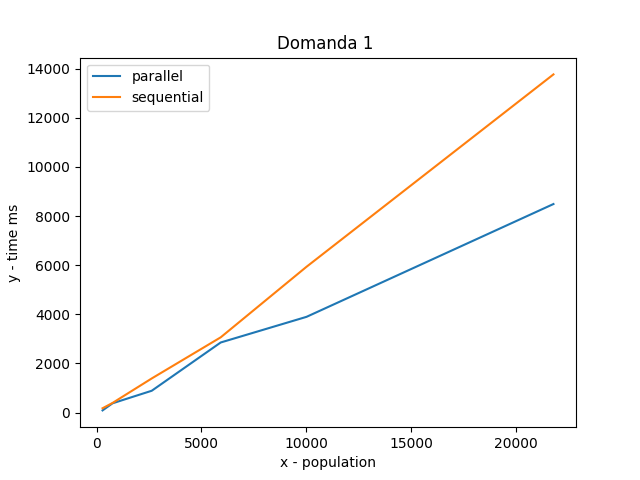
\includegraphics[width=0.7\linewidth, valign=t]{figures/domanda1}
		\caption*{Nel grafico vengono mostrati i tempi di esecuzione dell'algoritmo k-means parallelo e sequenziale, al variare della popolazione, calcolato su 50 cluster, 100 iterazioni e cutoff 20.}
	\end{figure}
\end{center}
\begin{center}
	\begin{figure}[H]
		\hspace*{1.5cm}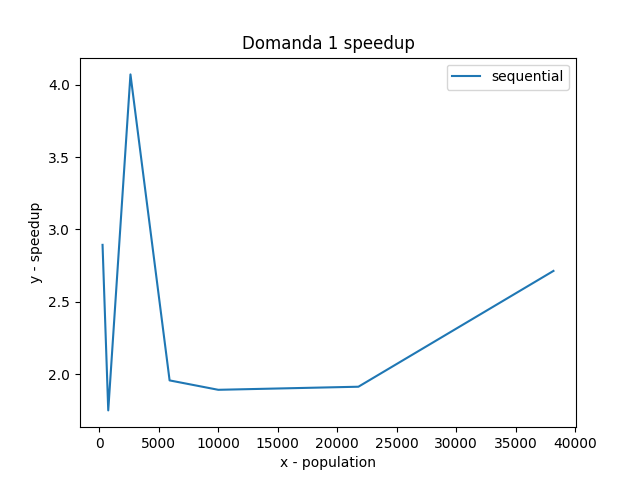
\includegraphics[width=0.7\linewidth, valign=t]{figures/domanda1speedup}
		\caption*{Il grafico mostra lo speedup calcolato come il rapporto tra i tempi dell'algoritmo k-means sequenziale e parallelo, al variare della popolazione. Dati i punti a disposizione non è possibile individuare una tendenza dell'andamento dello speedup.}
	\end{figure}
\end{center}

\vspace{-3cm}
\section*{Domanda 2}
\begin{center}
	\begin{figure}[H]
		\hspace*{1.5cm}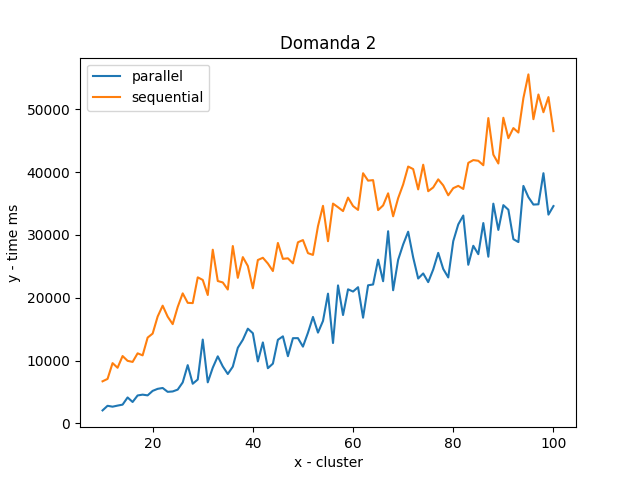
\includegraphics[width=0.7\linewidth, valign=t]{figures/domanda2}
		\caption*{Nel grafico vengono mostrati i tempi di esecuzione dell'algoritmo k-means parallelo e sequenziale, al variare del numero di cluster, calcolato sul dataset complessivo di 38183 punti, 100 iterazioni e cutoff 20, si può vedere come l'algoritmo parallelo abbia tempi sempre migliori rispetto la controparte sequenziale.}
	\end{figure}
\end{center}

\begin{center}
	\begin{figure}[H]
		\hspace*{1.5cm}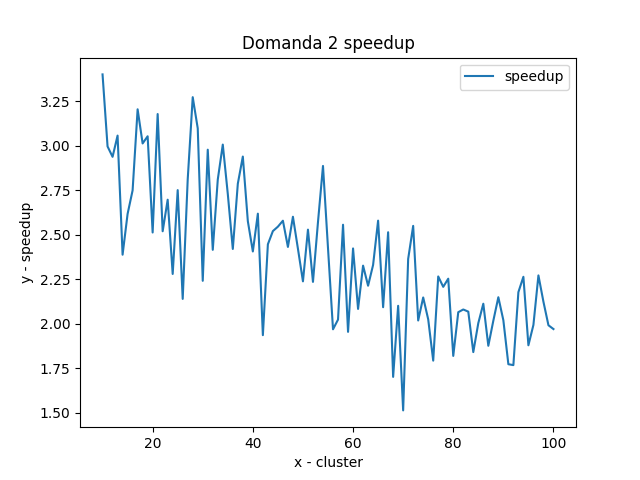
\includegraphics[width=0.7\linewidth, valign=t]{figures/domanda2speedup}
		\caption*{Il grafico mostra l'andamento dello speedup calcolato attraverso il rapporto tra i tempi dell'algoritmo k-means sequenziale e parallelo, al variare del numero di cluster. Si evince come lo speedup abbia un andamento descrescente, all'aumentare del numero dei cluster.}
	\end{figure}
\end{center}

\vspace{-3cm}
\section*{Domanda 3}
\begin{center}
	\begin{figure}[H]
		\hspace*{1.5cm}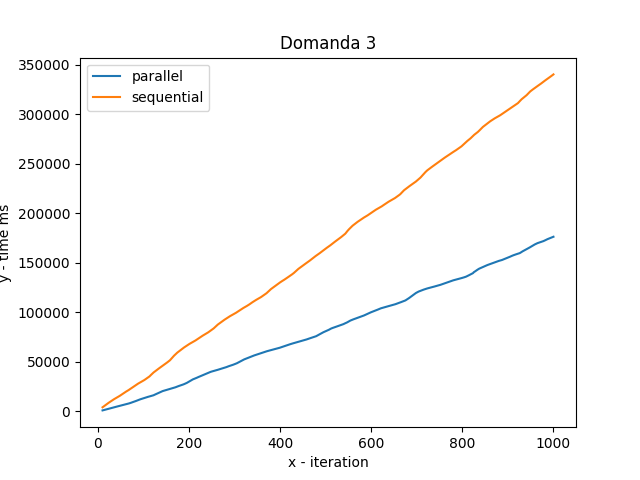
\includegraphics[width=0.7\linewidth, valign=t]{figures/domanda3}
		\caption*{Nel grafico vengono mostrati i tempi di esecuzione dell'algoritmo k-means parallelo e sequenziale, al variare del numero di iterazioni, calcolato sul dataset complessivo di 38183 punti, 50 cluster e cutoff 20, si può vedere come l'algoritmo parallelo abbia tempi sempre migliori rispetto la controparte sequenziale.}
	\end{figure}
\end{center}

\begin{center}
	\begin{figure}[H]
		\hspace*{1.5cm}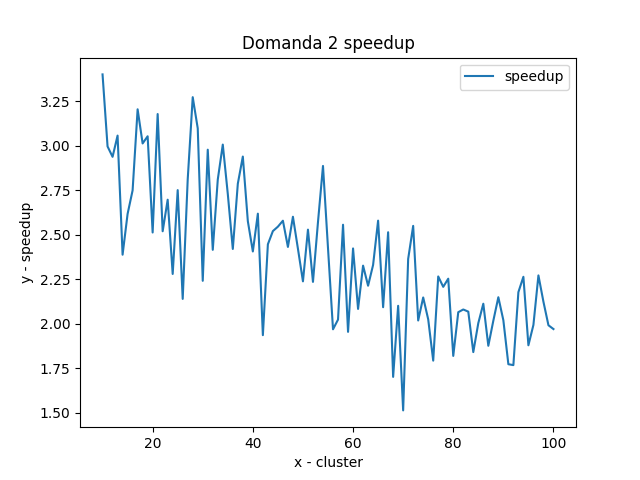
\includegraphics[width=0.7\linewidth, valign=t]{figures/domanda2speedup}
		\caption*{Il grafico mostra l'andamento dello speedup calcolato attraverso il rapporto tra i tempi dell'algoritmo k-means sequenziale e parallelo, al variare del numero di cluster. Si evince come lo speedup abbia un andamento descrescente, all'aumentare del numero dei cluster.}
	\end{figure}
\end{center}

\vspace{-3cm}
\section*{Domanda 4}
\begin{center}
	\begin{figure}[H]
		\hspace*{1.5cm}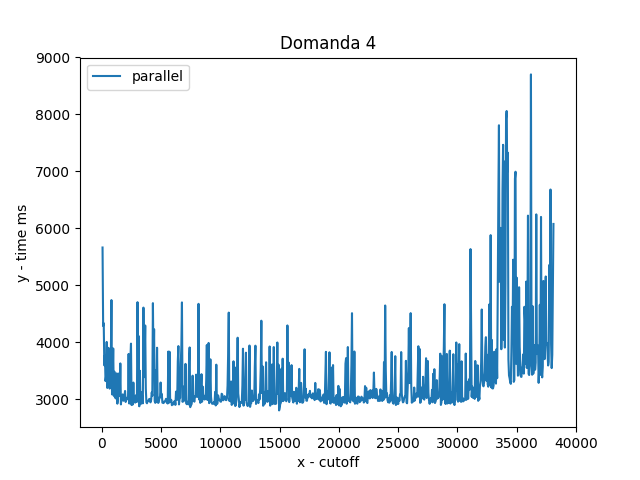
\includegraphics[width=0.7\linewidth, valign=t]{figures/domanda4}
		\caption*{Nel grafico vengono mostrati i tempi di esecuzione dell'algoritmo k-means parallelo, al variare del cutoff, calcolato sul dataset complessivo di 38183 punti, 50 cluster e 100 iterazioni, si può vedere come l'algoritmo parallelo dia il meglio di sè utilizzando un cutoff medio, ne troppo basso (parallelismo perfetto), ne troppo alto (praticamente sequenziale), favorendo quindi una versione ibrida.}
	\end{figure}
\end{center}

\begin{center}
	\begin{figure}[H]
		\hspace*{1.5cm}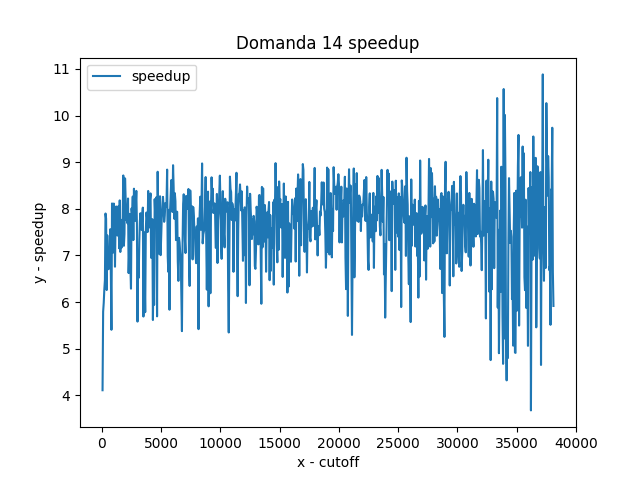
\includegraphics[width=0.7\linewidth, valign=t]{figures/domanda4speedup}
		\caption*{Il grafico mostra l'andamento dello speedup calcolato attraverso il rapporto tra i tempi dell'algoritmo k-means sequenziale e parallelo, al variare del cutoff. Si evince come lo speedup abbia un andamento lineare con tempi generalmente migliore nella parte centrale, evincendo come che una combinazione ibrida tra algoritmo parallelo e sequenziale sia quella con performance migliori.}
	\end{figure}
\end{center}

\section*{Domanda 5}
Il computer su cui sono stati eseguiti i test dispone del seguente processore: \textit{Intel(R) Core(TM) i7-2820QM CPU\\ Clockspeed: 2.3 GHz, Turbo Speed: 3.4 GHz\\ Number of Cores: 4 (2 logical cores per physical)}.


\end{document}


